% Practice Test 12 — Michigan Edition
% Questions: 30 (17 MC + 13 SA)
% Generated by scripts/generate_practice_tests.py

\begin{practiceQuestion}{1-3-q20}{sa}
\begin{questionText}
A store sells ribbon at a constant price per yard. If $3$ yards cost $\$4.50$, what is the constant of proportionality?
\end{questionText}
\correctAnswer{$k = \$1.50$ per yard}
\explanation{$k = \frac{4.50}{3} = 1.50$ dollars per yard.}
\end{practiceQuestion}

\begin{practiceQuestion}{1-5-q20}{sa}
\begin{questionText}
Two delivery services are proportional. Service A: $(2, 14)$. Service B: $(3, 18)$. Which has the higher rate and what is it?
\end{questionText}
\correctAnswer{Service A at $\$7$ per delivery}
\explanation{Service A: $k = \frac{14}{2} = 7$. Service B: $k = \frac{18}{3} = 6$. Service A has the higher rate at $\$7$.}
\end{practiceQuestion}

\begin{practiceQuestion}{1-6-q19}{sa}
\begin{questionText}
A recipe for $6$ servings uses $\frac{3}{4}$ cup of sugar. How much sugar is needed for $16$ servings?
\end{questionText}
\correctAnswer{$2$ cups}
\explanation{Per serving: $\frac{3}{4} \div 6 = \frac{3}{24} = \frac{1}{8}$ cup. For $16$: $\frac{1}{8} \times 16 = 2$ cups.}
\end{practiceQuestion}

\begin{practiceQuestion}{2-1-q21}{sa}
\begin{questionText}
$56$ is $80\%$ of what number?
\end{questionText}
\correctAnswer{$70$}
\explanation{Divide: $56 \div 0.80 = 70$.}
\end{practiceQuestion}

\begin{practiceQuestion}{2-5-q10}{mc}
\begin{questionText}
A car salesperson earns $4\%$ commission. She sold a car for $\$28{,}000$. How much commission did she earn?
\end{questionText}
\choiceA{$\$700$}
\choiceB{$\$1{,}120$}
\choiceC{$\$2{,}800$}
\choiceD{$\$11{,}200$}
\correctAnswer{B}
\explanation{$28{,}000 \times 0.04 = \$1{,}120$.}
\end{practiceQuestion}

\begin{practiceQuestion}{2-7-q29}{gsa}
\begin{questionText}
The table shows the results of a science experiment. Calculate the percent error for Trial 3 (round to the nearest tenth).

\begin{center}
\begin{tabular}{|l|c|c|c|}
\hline
 & \textbf{Predicted (g)} & \textbf{Actual (g)} & \textbf{Percent Error} \\
\hline
Trial 1 & $50$ & $48$ & $4.2\%$ \\
\hline
Trial 2 & $50$ & $55$ & $9.1\%$ \\
\hline
Trial 3 & $50$ & $44$ & ? \\
\hline
\end{tabular}
\end{center}
\end{questionText}
\correctAnswer{$\approx 13.6\%$}
\explanation{$\frac{|50 - 44|}{44} \times 100 = \frac{6}{44} \times 100 \approx 13.6\%$.}
\end{practiceQuestion}

\begin{practiceQuestion}{3-1-q23}{sa}
\begin{questionText}
Find two integers whose absolute values are both $7$.
\end{questionText}
\correctAnswer{$7$ and $-7$}
\explanation{$|7| = 7$ and $|-7| = 7$. A number and its opposite share the same absolute value.}
\end{practiceQuestion}

\begin{practiceQuestion}{3-2-q27}{gmc}
\begin{questionText}
Which number line correctly models $(-4) + (-3)$?

\begin{center}
\begin{tikzpicture}
  % Model A
  \node[left] at (-7.5,2) {\textbf{A:}};
  \draw[thick,->] (-7,2) -- (3,2);
  \foreach \x in {-6,...,2} \draw (\x,2.1) -- (\x,1.9) node[below] {\footnotesize $\x$};
  \draw[thick,->,funRed] (-4,2.4) -- (-7,2.4);

  % Model B
  \node[left] at (-7.5,0) {\textbf{B:}};
  \draw[thick,->] (-7,0) -- (3,0);
  \foreach \x in {-6,...,2} \draw (\x,0.1) -- (\x,-0.1) node[below] {\footnotesize $\x$};
  \draw[thick,->,funBlue] (-4,0.4) -- (-1,0.4);
\end{tikzpicture}
\end{center}
\end{questionText}
\choiceA{Model A}
\choiceB{Model B}
\choiceC{Both are correct}
\choiceD{Neither is correct}
\correctAnswer{A}
\explanation{$(-4) + (-3)$ means start at $-4$ and move $3$ units left (adding a negative). Model A shows the arrow going from $-4$ to $-7$, which is correct.}
\end{practiceQuestion}

\begin{practiceQuestion}{4-1-q20}{sa}
\begin{questionText}
Evaluate $-3x + 14$ when $x = -5$.
\end{questionText}
\correctAnswer{$29$}
\explanation{Substitute: $-3(-5) + 14 = 15 + 14 = 29$.}
\end{practiceQuestion}

\begin{practiceQuestion}{4-2-q10}{mc}
\begin{questionText}
Simplify $2.5a + 1.3 - 0.5a + 2.7$.
\end{questionText}
\choiceA{$2a + 4$}
\choiceB{$3a + 4$}
\choiceC{$2a - 4$}
\choiceD{$6$}
\correctAnswer{A}
\explanation{Combine variable terms: $2.5a - 0.5a = 2a$. Combine constants: $1.3 + 2.7 = 4$. Result: $2a + 4$.}
\end{practiceQuestion}

\begin{practiceQuestion}{5-2-q24}{sa}
\begin{questionText}
Solve $\dfrac{k}{8} + 9 = 15$.
\end{questionText}
\correctAnswer{$k = 48$}
\explanation{Subtract $9$: $\frac{k}{8} = 6$. Multiply by $8$: $k = 48$. Check: $\frac{48}{8} + 9 = 6 + 9 = 15$ \checkmark.}
\end{practiceQuestion}

\begin{practiceQuestion}{5-3-q15}{mc}
\begin{questionText}
Three friends split the cost of a gift equally. Each person also pays $\$4$ for wrapping. Each person pays $\$16$ total. What is the cost $c$ of the gift?
\end{questionText}
\choiceA{$c = 48$}
\choiceB{$c = 36$}
\choiceC{$c = 12$}
\choiceD{$c = 60$}
\correctAnswer{B}
\explanation{Each pays $\frac{c}{3} + 4 = 16$. This means $\frac{c}{3} = 12$, so $c = 36$. Or: total paid $= 3 \times 16 = 48$, wrapping $= 3 \times 4 = 12$, gift $= 48 - 12 = 36$.}
\end{practiceQuestion}

\begin{practiceQuestion}{5-4-q03}{mc}
\begin{questionText}
Solve $0.25n - 1.5 = 3.5$.
\end{questionText}
\choiceA{$n = 8$}
\choiceB{$n = 20$}
\choiceC{$n = 14$}
\choiceD{$n = 2$}
\correctAnswer{B}
\explanation{Add $1.5$: $0.25n = 5$. Divide by $0.25$: $n = 20$. Check: $0.25(20) - 1.5 = 5 - 1.5 = 3.5$ \checkmark.}
\end{practiceQuestion}

\begin{practiceQuestion}{5-5-q16}{mc}
\begin{questionText}
Solve $\dfrac{n}{5} - 2 > 4$.
\end{questionText}
\choiceA{$n > 10$}
\choiceB{$n > 30$}
\choiceC{$n > 1$}
\choiceD{$n < 30$}
\correctAnswer{B}
\explanation{Add $2$: $\frac{n}{5} > 6$. Multiply by $5$: $n > 30$.}
\end{practiceQuestion}

\begin{practiceQuestion}{5-6-q09}{mc}
\begin{questionText}
A parking garage charges $\$5$ per hour. You have $\$30$. Which inequality represents the hours $h$ you can park, and what does the graph look like?
\end{questionText}
\choiceA{$5h \leq 30$; closed circle at $6$, shade left from $0$ to $6$}
\choiceB{$5h < 30$; open circle at $6$, shade left}
\choiceC{$5h \geq 30$; closed circle at $6$, shade right}
\choiceD{$5h > 30$; open circle at $6$, shade right}
\correctAnswer{A}
\explanation{You can spend at most $\$30$: $5h \leq 30$, so $h \leq 6$. Closed circle at $6$, shade left (and $h \geq 0$).}
\end{practiceQuestion}

\begin{practiceQuestion}{6-2-q27}{gmc}
\begin{questionText}
The two rectangles below represent the same room drawn at two different scales. The original uses $1$ cm $= 6$ m. What scale does the new drawing use?

\begin{center}
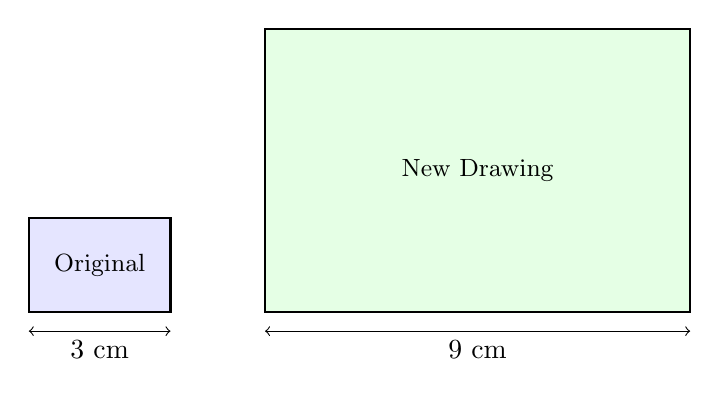
\begin{tikzpicture}[scale=0.6]
  % Original
  \draw[thick,fill=blue!10] (0,0) rectangle (3,2);
  \node at (1.5,1) {\small Original};
  \draw[<->] (0,-0.4) -- (3,-0.4);
  \node[below] at (1.5,-0.4) {$3$ cm};
  % New
  \draw[thick,fill=green!10] (5,0) rectangle (14,6);
  \node at (9.5,3) {\small New Drawing};
  \draw[<->] (5,-0.4) -- (14,-0.4);
  \node[below] at (9.5,-0.4) {$9$ cm};
\end{tikzpicture}
\end{center}
\end{questionText}
\choiceA{$1$ cm $= 2$ m}
\choiceB{$1$ cm $= 3$ m}
\choiceC{$1$ cm $= 6$ m}
\choiceD{$1$ cm $= 18$ m}
\correctAnswer{A}
\explanation{Scale ratio: $9 \div 3 = 3$. The new drawing is $3$ times bigger. Actual length: $3 \times 6 = 18$ m. New scale: $18 \div 9 = 2$ m per cm.}
\end{practiceQuestion}

\begin{practiceQuestion}{6-3-q15}{mc}
\begin{questionText}
Which condition makes it impossible to draw a triangle?
\end{questionText}
\choiceA{Sides $5$, $12$, $13$}
\choiceB{Sides $7$, $7$, $7$}
\choiceC{Sides $1$, $1$, $3$}
\choiceD{Sides $8$, $15$, $17$}
\correctAnswer{C}
\explanation{$1 + 1 = 2 < 3$. The triangle inequality fails. The other three sets all satisfy the triangle inequality.}
\end{practiceQuestion}

\begin{practiceQuestion}{6-4-q02}{mc}
\begin{questionText}
A triangle has angles $40°$, $60°$, and $80°$. How many different triangles can be drawn?
\end{questionText}
\choiceA{None}
\choiceB{Exactly one}
\choiceC{Exactly three}
\choiceD{Infinitely many}
\correctAnswer{D}
\explanation{AAA determines the shape but not the size. Infinitely many similar triangles of different sizes share these angle measures.}
\end{practiceQuestion}

\begin{practiceQuestion}{6-5-q23}{sa}
\begin{questionText}
A cylinder has a radius of $5$ cm and height of $12$ cm. It is sliced vertically through its center. What shape is the cross-section and what are its dimensions?
\end{questionText}
\correctAnswer{Rectangle; $10$ cm by $12$ cm}
\explanation{A vertical cut through the center of a cylinder produces a rectangle. Width = diameter = $2 \times 5 = 10$ cm. Height = $12$ cm.}
\end{practiceQuestion}

\begin{practiceQuestion}{7-3-q24}{sa}
\begin{questionText}
A circular plate has a diameter of $28$ cm. What is its area? Use $\pi \approx \frac{22}{7}$.
\end{questionText}
\correctAnswer{$616$ cm$^2$}
\explanation{$r = 14$ cm. $A = \frac{22}{7} \times 196 = 616$ cm$^2$.}
\end{practiceQuestion}

\begin{practiceQuestion}{7-4-q28}{gmc}
\begin{questionText}
The diagram shows a figure made of a rectangle and a triangle. What is the total area?

\begin{center}
\begin{tikzpicture}[scale=0.5]
  \fill[funBlue!20] (0,0) -- (10,0) -- (10,4) -- (5,7) -- (0,4) -- cycle;
  \draw[thick,funBlue] (0,0) -- (10,0) -- (10,4) -- (5,7) -- (0,4) -- cycle;
  \draw[dashed,gray] (0,4) -- (10,4);
  \draw[thick,funRed,<->] (0,-0.7) -- (10,-0.7);
  \node[below,funRed] at (5,-0.7) {$10$ m};
  \draw[thick,funRed,<->] (10.7,0) -- (10.7,4);
  \node[right,funRed] at (10.7,2) {$4$ m};
  \draw[thick,funRed,<->] (5,4) -- (5,7);
  \node[right,funRed] at (5,5.5) {$3$ m};
\end{tikzpicture}
\end{center}
\end{questionText}
\choiceA{$40$ m$^2$}
\choiceB{$55$ m$^2$}
\choiceC{$70$ m$^2$}
\choiceD{$85$ m$^2$}
\correctAnswer{B}
\explanation{Rectangle: $10 \times 4 = 40$ m$^2$. Triangle: $\frac{1}{2} \times 10 \times 3 = 15$ m$^2$. Total: $40 + 15 = 55$ m$^2$.}
\end{practiceQuestion}

\begin{practiceQuestion}{7-5-q05}{mc}
\begin{questionText}
A cube has a surface area of $150$ cm$^2$. What is the side length of the cube?
\end{questionText}
\choiceA{$5$ cm}
\choiceB{$10$ cm}
\choiceC{$25$ cm}
\choiceD{$15$ cm}
\correctAnswer{A}
\explanation{$SA = 6s^2$. So $s^2 = 150 \div 6 = 25$. Therefore $s = 5$ cm.}
\end{practiceQuestion}

\begin{practiceQuestion}{7-6-q30}{gsa}
\begin{questionText}
A rectangular prism-shaped fish tank is shown below. If water fills the tank to $\frac{3}{4}$ of its height, what is the volume of water in the tank?

\begin{center}
\begin{tikzpicture}[scale=0.35]
  % Tank outline
  \draw[thick,funBlue] (0,0) rectangle (10,8);
  \draw[thick,funBlue] (10,0) -- (14,3) -- (14,11) -- (10,8);
  \draw[thick,funBlue] (0,8) -- (4,11) -- (14,11);
  % Water level at 3/4
  \fill[cyan!30] (0,0) rectangle (10,6);
  \fill[cyan!20] (10,0) -- (14,3) -- (14,9) -- (10,6) -- cycle;
  \draw[dashed,funRed] (0,6) -- (10,6) -- (14,9);
  \node[left,funRed] at (0,6) {water};
  % Labels
  \draw[thick,funRed,<->] (0,-0.8) -- (10,-0.8);
  \node[below,funRed] at (5,-0.8) {$20$ cm};
  \draw[thick,funRed,<->] (-1,0) -- (-1,8);
  \node[left,funRed] at (-1,4) {$16$ cm};
  \draw[thick,funRed,<->] (14.5,3) -- (14.5,11);
  \node[right,funRed] at (14.5,7) {$16$ cm};
  \node[below right,funRed] at (12,1.5) {$10$ cm};
\end{tikzpicture}
\end{center}
\end{questionText}
\correctAnswer{$2{,}400$ cm$^3$}
\explanation{Full tank volume: $20 \times 10 \times 16 = 3{,}200$ cm$^3$. Water at $\frac{3}{4}$ height: $20 \times 10 \times 12 = 2{,}400$ cm$^3$.}
\end{practiceQuestion}

\begin{practiceQuestion}{8-1-q17}{mc}
\begin{questionText}
A doctor wants to study the effect of a new medicine on $10{,}000$ patients. She randomly selects $500$ patients for a trial. What is the sample size?
\end{questionText}
\choiceA{$10{,}000$}
\choiceB{$500$}
\choiceC{$10{,}500$}
\choiceD{$50$}
\correctAnswer{B}
\explanation{The sample size is the number of individuals selected — $500$ patients.}
\end{practiceQuestion}

\begin{practiceQuestion}{8-3-q07}{mc}
\begin{questionText}
Two box plots are drawn on the same number line. Box plot A is entirely to the right of box plot B. What does this tell you?
\end{questionText}
\choiceA{Group A has more data}
\choiceB{All values in Group A are greater than all values in Group B}
\choiceC{Group A has no overlap with Group B}
\choiceD{Both B and C}
\correctAnswer{D}
\explanation{If box plot A is entirely to the right, every value in A exceeds every value in B, so there is no overlap.}
\end{practiceQuestion}

\begin{practiceQuestion}{8-4-q03}{mc}
\begin{questionText}
Group A has a mean of $50$ and a MAD of $3$. Group B has a mean of $60$ and a MAD of $3$. The difference in means expressed in MADs is:
\end{questionText}
\choiceA{$\frac{10}{3} \approx 3.3$ MADs}
\choiceB{$10$ MADs}
\choiceC{$3$ MADs}
\choiceD{$30$ MADs}
\correctAnswer{A}
\explanation{Difference $= 60 - 50 = 10$. In MADs: $\frac{10}{3} \approx 3.3$.}
\end{practiceQuestion}

\begin{practiceQuestion}{9-1-q21}{sa}
\begin{questionText}
A standard number cube is rolled. What is the probability of rolling a number greater than $2$? Write your answer as a fraction.
\end{questionText}
\correctAnswer{$\frac{2}{3}$}
\explanation{Numbers greater than $2$: $3, 4, 5, 6$ — that is $4$ out of $6$. $P = \frac{4}{6} = \frac{2}{3}$.}
\end{practiceQuestion}

\begin{practiceQuestion}{9-4-q15}{mc}
\begin{questionText}
Which of these is NOT a valid probability model?
\end{questionText}
\choiceA{$P(A) = 0.5$, $P(B) = 0.5$}
\choiceB{$P(A) = 0.7$, $P(B) = 0.2$, $P(C) = 0.1$}
\choiceC{$P(A) = 0.6$, $P(B) = 0.6$}
\choiceD{$P(A) = 1$}
\correctAnswer{C}
\explanation{$0.6 + 0.6 = 1.2 > 1$. The probabilities must sum to exactly $1$.}
\end{practiceQuestion}

\begin{practiceQuestion}{9-6-q25}{sa}
\begin{questionText}
Three coins are flipped. What is the probability of getting exactly $1$ head? Write your answer as a fraction in simplest form.
\end{questionText}
\correctAnswer{$\frac{3}{8}$}
\explanation{Outcomes with exactly $1$ head: HTT, THT, TTH — that is $3$ out of $8$. $P = \frac{3}{8}$.}
\end{practiceQuestion}

\begin{practiceQuestion}{9-7-q14}{mc}
\begin{questionText}
Mia uses a random number generator to produce digits $0$--$9$. She runs $20$ trials to simulate a $40\%$ chance of an event. In her simulation, the event happens $10$ times. What is the experimental probability?
\end{questionText}
\choiceA{$0.20$}
\choiceB{$0.40$}
\choiceC{$0.50$}
\choiceD{$0.10$}
\correctAnswer{C}
\explanation{$P = \frac{10}{20} = 0.50$. This is higher than the theoretical $0.40$, but with only $20$ trials, variation is expected.}
\end{practiceQuestion}
